\chapter{بهبود تشخیص اخبار جعلی با فراداده‌های حاصل از پردازش زبان}
\section{انگیزه}
در بسیاری از موارد  صحت‌سنجی یک خبر با استفاده از متن خبر کار بسیار دشوار و پیچیده‌ای است. اما بعضی‌از فراداده‌های مرتبط با اخبار می‌تواند در تشخیص صحت این دسته از اخبار به ما کمک کند. در این فاز، به بررسی تأثیر استفاده از سه فراداده موضوع خبر، احساس خبر و موجودیت‌های نامدار موجود در خبر می‌پردازیم. با تحلیل و بررسی اخبار جعلی می‌توانیم دریابیم که آیا بعضی از موضوعات مثلاً سیاسی یا اجتماعی نسبت ‌به موضوعات دیگر مانند ورزشی بیشتر در معرض جعل خبر قرار دارد و خبر جعلی بیشتر در این موضوع مشخص تولید می‌شود یا خیر. دلیل این موضوع را می‌توان به‌دلیل تأثیرگذاری زیاد اخبار سیاسی و اجتماعی مطرح کرد. در صورت تأیید این فرضیه، انتظار می‌رود با دانستن موضوع هر خبر، بتوانیم درکنار متن خبر، با دقت بیشتری میزان جعلی‌بودن آن خبر را مشخص کنیم. علاوه بر این، یافتن موجودیت‌های نامدار و حس متن در هر خبر نیز می‌تواند اطلاعات نسبتاً مناسبی در مورد میزان صحت آن خبر ارائه دهد. در صورت تأیید این فرضیه نیز می‌توان حدس زد وجود اسامی خاص افراد، سازمان‌ها، مکان‌ها و ... در متن و یا حس مثبت یا منفی در متن می‌تواند به تشخیص جعلی‌بودن آن کمک کند. در ادامه این فصل به پردازش‌های متنی داده‌های خبری شامل دسته‌بندی موضوعی، تشخیص موجودیت‌های نامدار و تحلیل احساسات می‌پردازیم و در نهایت تأثیر آن‌ها را بررسی می‌نماییم.

\section{دسته‌بندی موضوعی اخبار}
\label{section.cat_detail}
همانطور که در بخش \ref{section.cat} به‌طور مفصل درمورد استخراج موضوع اخبار گفته شد، دو رویکرد اصلی برای استخراج موضوعات اخبار وجود دارد که ما بتوانیم با استفاده از آن‌ها دقت تشخیص اخبار جعلی را بالاتر ببریم. رویکرد اول استفاده از دسته‌بندی با مربی براساس ۶ کلاس مختلف است. در این حالت ما با استفاده از یک مدل آموزش‌دیده‌شده با پیکره بزرگ همشهری \citep{aleahmad2009hamshahri}، اخبار موجود در مجموعه دادگان «تاج» را برچسب می‌زنیم و از این برچسب به‌عنوان یک ویژگی جدا به‌صورت یک بردار ۶ بعدی در کنار ویژگی‌های مرتبط با متن مورد استفاده قرار می‌دهیم. رویکرد دوم استفاده از یک روش دسته‌بندی موضوعی بدون مربی 
	براساس روش تخصیص نهان دیریکله\LTRfootnote{Latent Dirichlet Allocation} \citep{blei2003latent} می‌باشد. 
	
در این روش یک بردار 50 بعدی که نماینده احتمال تعلق به هر موضوع است در کنار ویژگی‌های متنی آن برای تشخیص جعلی‌بودن خبر استفاده می‌شود.

\section{تشخیص موجودیت‌های نامدار}
شناسایی موجودیت­‌های نامدار در پردازش زبان طبیعی به عملیاتی گفته می‌­شود که در آن تمامی­ اسامی خاص موجود در متن شناسایی و استخراج می‌گردد و به مقولات ازپیش ‌تعریف‌شده‌ای مانند اسم افراد، سازمان‌ها، مکان‌ها و ... دسته بندی می‌شود به این صورت که متن را بر اساس واژه‌ها قطعه‌بندی نموده و با برچسب‌زنی، عبارات حاوی موجودیت‌های نامدار را مشخص می‌نماییم.

در واقع مسأله تشخیص موجودیت‌های نامدار در متن عموماً به دو زیر‌مسأله تشخیص و دسته‌بندی موجودیت‌ها تقسیم می‌شود. اسامی خاصی که تشخیص داده می‌شود و همچنین قالبی که برای دسته‌بندی آن‌ها به‌کار می‌رود وابسته به نوع کاربرد آن خواهد‌ بود. در سامانه‌های تشخیص موجودیت‌های نامدار، بیشتر بر روی تشخیص اسامی اشخاص، مکان‌­ها و سازمان‌هایی که در یک متن ذکر شده‌است تمرکز است \citep{chen2015}.

نیاز به شناسایی موجودیت­‌های نامدار در دنیای امروز که عصر ارتباطات و اطلاعات است به‌شدت احساس می‌­شود. شناسایی موجودیت‌­های نامدار برای جستجوهای معنادار\LTRfootnote{Semantic Search}، ترجمه ماشینی\LTRfootnote{Machine Translation}، استخراج اطلاعات از متن\LTRfootnote{Information Extraction}، مرجع‌یابی در متن\LTRfootnote{Co-reference Resolution}، سیستم­‌های پرسش و پاسخ\LTRfootnote{Question Answering Systems} ، سیستم‌های خبره\LTRfootnote{Expert Systems} ، کشف دانش\LTRfootnote{Knowledge Discovery} ، مدیریت دانش\LTRfootnote{Knowledge Management}، تحلیل احساسات\LTRfootnote{Sentiment Analysis}، بازیابی اطلاعات\LTRfootnote{Information Retrieval}، تحلیل خبر\LTRfootnote{News Analysis} و بسیاری دیگر از شاخه های مرتبط با پردازش زبان­ طبیعی کاربرد دارد. اینکه سیستم چه نوع موجودیتی را تشخیص دهد و یا به بیان دیگر دسته‌های معنایی مورد نظرش چه باشند، وابسته به زمینه کاربردی سیستم است \citep{ABDALLAH201734}.\\
به‌عنوان مثال، شناسایی موجودیت‌های نامدار در علم زیست‌شناسی می‌­تواند تشخیص اسامی وابسته به انواع پروتئین­، دی‌ان‌­ای، نوع سلول و غیره باشد. در حوزه پزشکی می‌تواند تشخیص انواع بیماری، دارو، و مراکز درمانی باشد. در حوزه تجارت نام شرکت‌­ها و مؤسسات، تراکنش­‌های مالی، بورس و غیره باشد؛ یا به‌صورت خیلی خاص  تنها برای تشخیص اسامی شرکت­‌های تولید کننده فولاد به‌کار رود.

یکی از کاربردهای تشخیص موجودیت‌­های نامدار در ترجمه ماشینی رفع ابهام از ترجمه و افزایش دقت آن است. به‌عنوان مثال، اگر در متنی واژه \lr{Apple} به‌عنوان موجودیت نامدار شناخته شده باشد و دارای برچسب باشد، در این صورت در هنگام ترجمه به‌عنوان شرکت «اپل» شناخته می‌­شود و معنای «سیب» نخواهد داشت. در مثالی دیگر، در ترجمه فارسی به انگلیسی می‌­توان به واژه «زیبا» اشاره کرد. اگر این واژه اسم فرد و موجودیت نامدار باشد، نیاز به ترجمه ندارد، و درغیراین‌­صورت باید به واژه \lr{Beautiful} ترجمه شود \citep{Hussain2016}.

به طور کلی از دو روش قاعده‌مند و آماری برای تشخیص موجودیت‌­های نامدار استفاده می‌­شود \citep{Jurafsky2009}. در روش‌­های قاعده‌مند، قوانینی تعریف می‌­شود که براساس آنها موجودیت‌­های نامدار تشخیص داده می‌­شود. در روش آماری، از تکنیک­‌های یادگیری ماشین برای دسته­‌بندی موجودیت­‌های نامدار به هر مقوله استفاده می‌­شود. استفاده از روش­‌های دسته‌بندی بانظارت در این قسمت سبب می‌­شود  با استفاده از پیکره‌هایی که موجودیت‌­های نامدار  در آن‌ها برچسب‌گذاری شده‌است  مدلی را آموزش داد، و با استفاده از آن مدل بتوان متن بدون برچسب را برچسب‌گذاری نمود و موجودیت‌های نامدار را در آن‌ها به‌طور خودکار تشخیص داد. در پروژه حاضر، برای ساخت سامانه تشخیص موجودیت­‌های نامدار از روش­‌های یادگیری ماشین بانظارت و مبتنی ‌بر یادگیری عمیق استفاده می‌کنیم.

\subsection{دادگان}
برای یادگیری مدل، نیازمند پیکره‌­ای برای آموزش شبکه عصبی هستیم. از جمله دادگان موجود در زمینه تشخیص موجودیت­‌های نامدار در زبان فارسی، پیکره‌های موجویت‌­های نامدار آرمان \citep{poostchi2016personer}، پیما \citep{shahshahani2019peyma} و درخت‌بانک هسته‌بنیان فارسی \citep{ghayoomi2012} می‌­باشد. در پیکره سوم  تنها موجودیت‌­های نامدار مربوط به نام اشخاص، موقعیت­‌های مکانی و اسامی مربوط به سازمان‌­ها برچسب‌گذاری شده‌است. درحالی‌که در پیکره اول، علاوه‌بر این سه برچسب، اسامی رویدادها، امکانات و محصولات نیز مشخص شده و در پیکره دوم نیز زمان، تاریخ، مبالغ مالی و درصد برچسب‌گذاری شده‌است.  این در حالی است که در بسیاری از کاربردهای تشخیص موجودیت‌­های نامدار، مانند سیستم‌­های پرسش و پاسخ و یا تحلیل اخبار و ...، نیازمند پوشش موجودیت­‌های نامدار بیشتری مانند زبان‌­ها، ملیت‌­ها، رخدادها، مشاغل، کتاب‌­ها، اسامی فیلم‌­ها، تاریخ­‌ها، مذاهب، زمینه‌های علمی و دانش‌­ها، روزنامه‌­ها و سایر اسامی خاص در زبان هستیم.

ازآنجاکه در پیکره­‌های مذکور این موارد پوشش داده نشده بود، برای به‌کاربردن ویژگی‌های حاصل از تشخیص موجودیت­‌های نامدار در تشخیص اخبار جعلی، از پیکره‌­ موجودیت‌های نامدار تهیه‌شده در آزمایشگاه پردازش زبان طبیعی دانشگاه صنعتی امیرکبیر که حاوی پانزده برچسب موجودیت‌­های نامدار است استفاده شده‌است \citep{momtazi2020named}. این دادگان که شامل حدود ۳۰۰۰ چکیده ویکی‌پدیا بوده و به‌صورت دستی برچسب‌خورده است می‌­تواند در این پژوهش مورد استفاده قرار بگیرد و سبب شود تجزیه­ و­ تحلیل و نتیجه‌گیری از داده‌ها را با دقت بالاتری انجام دهد. 

در ادامه، به توضیح اجمالی برچسب‌های این پیکره می‌پردازیم. واژه‌ها گردآوری‌شده از ویکی‌پدیای فارسی برای آموزش سیستم نیازمند برچسب‌گذاری با نمادهایی است که هر کدام به یک نوع از موجودیت‌­های نامدار اشاره دارد. تعداد کل برچسب­‌های استفاده‌شده در دادگان ۳۱ برچسب است که برای مشخص‌کردن ۱۵ نوع موجودیت متفاوت که شامل اسم شخص مفرد، اسم شخص جمع، موقعیت مکانی، اسم سازمان، زبان، ملیت، رخداد، شغل، کتاب، اسم فیلم، تاریخ، مذهب، عنوان علمی و دانش، روزنامه و سایر اسامی خاص ذکرنشده در زبان فارسی می‌باشد استفاده شده‌است. همچنین برای واژه‌هایی که جزو موجودیت­‌های نامدار نیست نیز علامتی در نظر گرفته شده‌است. در این دادگان، برای تعیین اسم خاص اشخاص از دو برچسب مختلف استفاده شده‌است که یکی برای تعیین اسامی خاص مفرد و معمول به‌کار می‌­رود و با علامت \lr{PEI} مشخص شده و دیگری برای اسامی خاص که به‌صورت جمع استفاده می‌شود کاربرد دارد. این موارد با برچسب \lr{PEG} مشخص شده‌است.

اسم شخص جمع به تمامی اسامی گفته می‌شود که اسم مفرد آن نوعی موجودیت باشد. به‌­عنوان مثال واژه‌های «مسلمان»، «معلم» و «ایرانی» به‌­ترتیب برچسب‌­های مذهب، شغل و ملیت می‌­گیرند و اسم جمع این واژه‌ها یعنی «مسلمانان»، «معلمان» و «ایرانیان» \lr{PEG} محسوب می‌­شود. همین‌طور واژه «ابوالفضل بلعمی» دارای برچسب \lr{PEI} است و به طبع آن واژه‌های «خاندان بلعمی» و یا «بلعمیان» برچسب \lr{PEG} دارد. جدول \ref{table.NER_tags} به تفضیل به شرح و بررسی برچسب­‌های استفاده‌شده برای دادگان می‌پردازد.

\begin{table}
	\caption{راهنمای برچسب واژگان}
	\label{table.NER_tags}
	\begin{center}
		\small
		\begin{tabular}{|P{1.2cm}|P{2cm}|P{2cm}|P{8cm}|}
			\hline
			برچسب & تعریف انگلیسی برچسب & تعریف فارسی برچسب & توضیحات \\
			\hline
			\lr{O} & \lr{Out} &
			هیچ & واژه مورد نظر از موجودیت‌های نامدار نیست. \\
			\hline
			\lr{PEI} & \lr{Person Individual} &
			شخص مفرد & این علامت به نام شخص اشاره دارد. \\
			\hline
			\lr{PEG} & \lr{Person Group} &
			اسم خاص گروه & این علامت به موجودیت نامداری اشاره دارد که به‌صورت جمع آمده‌است.\\
			\hline
			\lr{LOC} & \lr{Location} &
			موقعیت مکانی & واژه مورد نظر این برچسب به موقعیت مکانی خاصی اشاره دارد. \\
			\hline
			\lr{ORG} & \lr{Organization} &
			سازمان  & اسامی سازمان‌­ها و مؤسسات مختلف با این برچسب نشان داده می‌­شود. \\
			\hline
			\lr{LAN} & \lr{Language} &
			زبان & این برچسب نشان‌دهنده زبان‌­های مختلف است. \\
			\hline
			\lr{NAT} & \lr{Nationality} &
			ملیت & ملیت­‌های مختلف با این علامت تعیین می‌­شود. \\
			\hline
			\lr{EVN} & \lr{Events} &
			رخدادها & رخدادها و وقایع خاص را با این برچسب نشان دادیم. \\
			\hline
			\lr{JOB} & \lr{Job} &
			شغل & این برچسب نمایانگر مشاغل است. \\
			\hline
			\lr{BOK} & \lr{Book} &
			کتاب & اسامی کتاب‌­ها با این برچسب مشخص می‌شود. \\
			\hline
			\lr{FLM} & \lr{Film} &
			فیلم & نام فیلم‌­های مختلف با این برچسب تعیین می‌­شود. \\
			\hline
			\lr{DTE} & \lr{Date} &
			تاریخ & برای نشان‌دادن تاریخ و دوره‌های مختلف از برچسب استفاده شده‌است. \\
			\hline
			\lr{REL} & \lr{Religion} &
			مذهب & این برچسب تعیین‌کننده مذاهب مختلف است. \\
			\hline
			\lr{FLD} & \lr{Field} &
			زمینه & زمینه‌ها و دانش‌­های مختلف با این برچسب تعیین گردیده‌است. \\
			\hline
			\lr{MAG} & \lr{Magazine} &
			روزنامه و مجله & اسامی روزنامه‌ها و مجلات با این برچسب آمده‌است. \\
			\hline
			\lr{OTH} & \lr{Other} &
			سایرین & اگر واژه‌ای به‌عنوان موجودیت نامدار باشد ولی در بین موجودیت­‌های معرفی‌شده در بالا نباشد با این برچسب مشخص می‌­شود. \\
			\hline
			
		\end{tabular}
	\end{center}
\end{table}

\subsection{مدل}
اساس خیلی از برنامه‌ها قابلیت پیش‌بینی دنباله‌ای از متغیر‌ها است که به همدیگر وابسته هستند. این مسئله کاربرد زیادی در حوزه‌های مختلف پردازش متن دارد. برای تشخیص موجودیت‌های نامدار باید دنباله واژه‌ها را مدل کرد و برای هر واژه یک خروجی ساخت. برای مدل‌سازی دنباله‌ها روش‌های متعددی وجود دارد که در این میان رویکرد مبتنی‌بر شبکه عصبی بازگشتی با میدان شرطی تصادفی بیشترین محبوبیت را دارد. این مدل یک شبکه عصبی بازگشتی دوطرفه به‌‌علاوه یک لایه میدان تصادفی شرطی در انتها است. شبکه عصبی بازگشتی برای یک واژه اطلاعاتی در مورد بافت آن واژه و واژه‌ها قبل از آن مهیا می‌کند و در حالت دوطرفه علاوه بر واژه‌های قبل، واژه‌های بعد از آن را هم در نظر می‌گیرد. لایه میدان تصادفی شرطی برای پیش‌بینی برچسب هر واژه، برچسب واژه‌های دیگر را نیز در نظر می‌گیرد.

مشابه رویکردی که در بازنمایی متون در تشخیص اخبار جعلی داشتیم در بخش تشخیص موجودیت‌های نامدار نیز بازنمایی عصبی با استفاده از مدل‌های زبانی مبتنی بر معماری انتقال‌دهنده‌ مورد استفاده قرار گرفته است. برت می‌تواند برای طیف گسترده‌ای از کارهای زبانی مورد استفاده قرار گیرد‌، در حالی که فقط یک لایه به مدل اصلی اضافه می‌شود. در تشخیص موجودیت‌های نامدار‌ با استفاده از برت می‌توان با تغذیه بردار خروجی هر نشانه در یک لایه طبقه‌بندی که برچسب موجودیت نامدار را پیش‌بینی می‌کند‌، یک مدل تشخیص موجودیت نامدار آموزش داد.

اگرچه مدل حاصل از ترکیب شبکه عصبی بازگشتی و میدان شرطی تصادفی در پژوهش‌های مختلف به نتایج بهتری نسبت‌به مدل‌های قبلی رسیده‌است \citep{huang2015bidirectional}، با استفاده از مدل‌های مبتنی‌بر ترانسفورمر برای بازنمایی متن ویژگی‌های مورد استفاده در شبکه \lr{BiLSTM} در بخش بازنمایی مورد توجه قرار می‌گیرد و استفاده از شبکه \lr{BiLSTM} پس‌از بازنمایی به دقت مدل نمی‌افزاید \citep{Thesis_abdolah}. در نتیجه، در پژوهش حاضر برای تشخیص موجودیت‌های نامدار از شبکه برت به‌همراه یک لایه میدان شرطی تصادفی استفاده می‌کنیم. 

درمیان مدل‌های مبتنی‌بر برت که برای زبان فارسی قابل استفاده است، مدل ایکس.ال.ام-روبرتا به نتایج قابل قبولی در این زمینه رسیده‌است و براساس نتایج گزارش‌شده توسط \cite{Thesis_abdolah} از این مدل برای تشخیص موجودیت نامدار استفاده می‌شود.

\section{تحلیل احساسات}
نظرکاوی یا تحلیل احساسات، مطالعه محاسباتی نظرات کاربران حول محصولات، خدمات، سازمان‌ها، اشخاص، رویدادها و جنبه‌های مختلف آن است. در سال‌های اخیر این حوزه یکی از حوزه‌های پژوهشی فعال در پردازش زبان‌های طبیعی بوده است. نظرکاوی در سطوح مختلف سند، جمله و جنبه مورد مطالعه قرار گرفته‌است. در حوزه کالا و خدمات هنگام تصمیم‌گیری عقاید دیگران تأثیر به‌سزایی در تصمیم نهایی دارد. در دنیای واقعی، شرکت‌ها همواره نیازمند عقاید مردم برای بهبود کیفیت و توسعه خدمات خود است. در دنیای نشر خبر، سوگیری احساسی اخبار یکی از جنبه‌های مؤثر در تحلیل خبر می‌باشد. مثبت یا منفی بودن یک خبر می‌تواند جنبه‌های مختلفی از تحلیل آن خبر را فراهم آورد. درحال‌حاضر داده‌های متنی  بخش عظیمی از شبکه‌های اجتماعی، فروشگاهای اینترنتی و انواع مختلف سامانه‌های ارتباطی را در بر گرفته‌است. از این داده‌ها می‌توان در راستای درک احساسات کاربران به مطالب مختلف مانند یک محصول، یک نوشته موضوعی و ... استفاده کرد. 

نظر‌کاوی در سال 2002 توسط \citet{pang2002} معرفی شد. با روی‌کارآمدن شبکه‌های اجتماعی و تأثیر روزافزون آن‌ها بر زندگی مردم، اهمیت نظر‌کاوی و کاربردهای آن بیشتر مشخص گردید. باتوجه‌به این که افراد با حضور در این شبکه‌ها به بیان نظرات، عقاید و دیدگاه‌های خود درباره کلیه مسائل سیاسی، اجتماعی، فرهنگی، اقتصادی و حتی فردی می‌پردازد، تحلیل احساسات بیشتر از هر چیز در شبکه‌های اجتماعی مورد توجه قرار گرفته‌است. در کنار بستری که در شبکه‌های اجتماعی فراهم شده‌است، متون موجود در داده‌های خبری نیز می‌توانند دارای حس مثبت یا منفی باشد که به تحلیل آن کمک می‌نماید.

برای استفاده از تحلیل احساسات در تشخیص اخبار جعلی، تحلیل احساس در سطح سند مورد توجه این پژوهش قرار گرفته‌است و با بهره‌گیری از یک مدل مبتنی‌بر یادگیری عمیق حس موجود در متن به‌صورت یک بردار دو بعدی برای حس مثبت و منفی مشخص می‌گردد. خروجی این مدل به‌عنوان یکی از ویژگی‌های ورودی در مدل تشخیص اخبار جعلی استفاده خواهد شد.

\subsection{مدل}
برای پیاده‌سازی بخش تشخیص احساسات از شبکه پیچشی استفاده شده‌است. باتوجه‌ به این که پایه اصلی تحلیل احساسات دسته‌بندی متون است، ساختار شبکه پیچشی مورد استفاده در این بخش مشابه شبکه پیچشی‌ای است که در تشخیص خبر جعلی مورد استفاده قرار گرفته‌است و توضیحات آن در بخش ۳-۲-۲ گزارش فاز اول آمده‌است.  بازنمایی مورد استفاده در این شبکه نیز بازنمایی ایکس.ال.ام-روبرتا می‌باشد.

\section{نتایج حاصل از استفاده از پردازش‌های متنی در تشخیص اخبار}
در فصل ۳، با بررسی و مقایسه مدل‌های از پیش آموزش دیده، بهترین مدل بازنمایی اخبار ورودی را انتخاب کردیم. در این بخش می‌خواهیم با استفاده از هر دو مدل دسته‌بند شبکه پیشرو پرسپترون و شبکه عصبی پیچشی و استفاده از مدل پارس‌برت برای بازنمایی اخبار، از فراداده‌هایی مانند موضوع خبر، موجودیت‌های نامدار و یا حس متن در کنار بردار بازنمایی متن خبر استفاده کنیم.

همانطور که در بخش \ref{section.cat_detail} گفته شد برای استفاده از ویژگی موضوع خبر در رویکرد اول  یک بردار ویژگی ۶ بعدی حاصل از دسته‌بندی موضوعی اخبار و در رویکرد دوم یک بردار ویژگی ۵۰ بعدی حاصل از تخصیص نهان دیریکله خواهیم داشت. بازنمایی خروجی تحلیل احساس نیز یک بردار دو بعدی است که هر درایه آن نشان‌دهنده مثبت و یا منفی بودن آن خبر است. همچنین، اطلاعات مربوط به موجودیت‌های نامدار موجود در یک خبر با استفاده از یک بردار شامل ۱۵ ویژگی بازنمایی می‌شود. برای نمونه،  در جدول \ref{table.ner_example} نمونه‌ای از یک جمله برچسب‌گذاری‌شده نمایش داده شده‌است. در بردار ۱۵تایی حاصل از این جمله، درایه مربوط به موجودیت کتاب مقدار ۲، درایه‌های مربوط به موجودیت‌های زبان، شخص مفرد، شغل و تاریخ مقدار ۱، و سایر درایه‌ها مقدار صفر خواهد داشت. 
\begin{table}[h!]
	\caption{مثال از یک جمله برچسب‌خورده توسط مدل تشخیص موجودیت نامدار}
	\label{table.ner_example}
	\begin{center}
		\begin{tabular}{|c|c|}
			\hline
			واژه & برچسب \\
			\hline
			\hline
			کتاب &\lr{b-BOK} \\
			گلستان & \lr{i-BOK} \\
			و & \lr{O} \\
			کتاب & \lr{b-BOK} \\
			بوستان & \lr{i-BOK} \\
			از & \lr{O} \\
			شاهکارهای & \lr{O} \\
			ادب & \lr{O} \\
			فارسی & \lr{b-LAN} \\
			و & \lr{O} \\
			اثر & \lr{O} \\
			سعدی & \lr{b-PEI} \\
			شاعر & \lr{b-JOB} \\
			قرن & \lr{b-DTE} \\
			ششم & \lr{i-DTE} \\
			هجری & \lr{i-DTE} \\
			است & \lr{O} \\
			\hline
			
		\end{tabular}
	\end{center}
\end{table}


به‌منظور استفاده از ویژگی‌های فراداده‌های مختلف،  بردار‌های این ویژگی‌ها را ابتدا به یک لایه چگال با همان تعداد نورون وارد می‌کنیم و پس‌از‌ آن بردار خروجی لایه چگال را به انتهای بردار ویژگی‌های نهایی استخراج‌شده از متن اخبار الحاق می‌کنیم. درنهایت پس‌ از ساخت بردار ویژگی جدید، شامل ویژگی‌های متن و فراداده‌ها، آن را وارد یک لایه پرسپترون می‌کنیم تا برچسب اخبار مشخص شود. شِمای کلی مدل ارائه‌شده برای استفاده از تمام فراداده‌ها در کنار ویژگی‌های مبتنی بر بافت اخبار در شکل \ref{fig.all_features} ارائه شده است. همچنین، شکل \ref{fig.cnn_ner}  معماری شبکه عصبی پیچشی را در حالت استفاده از بردار فراداده‌ها نشان می‌دهد. 

\begin{figure}[h!]
	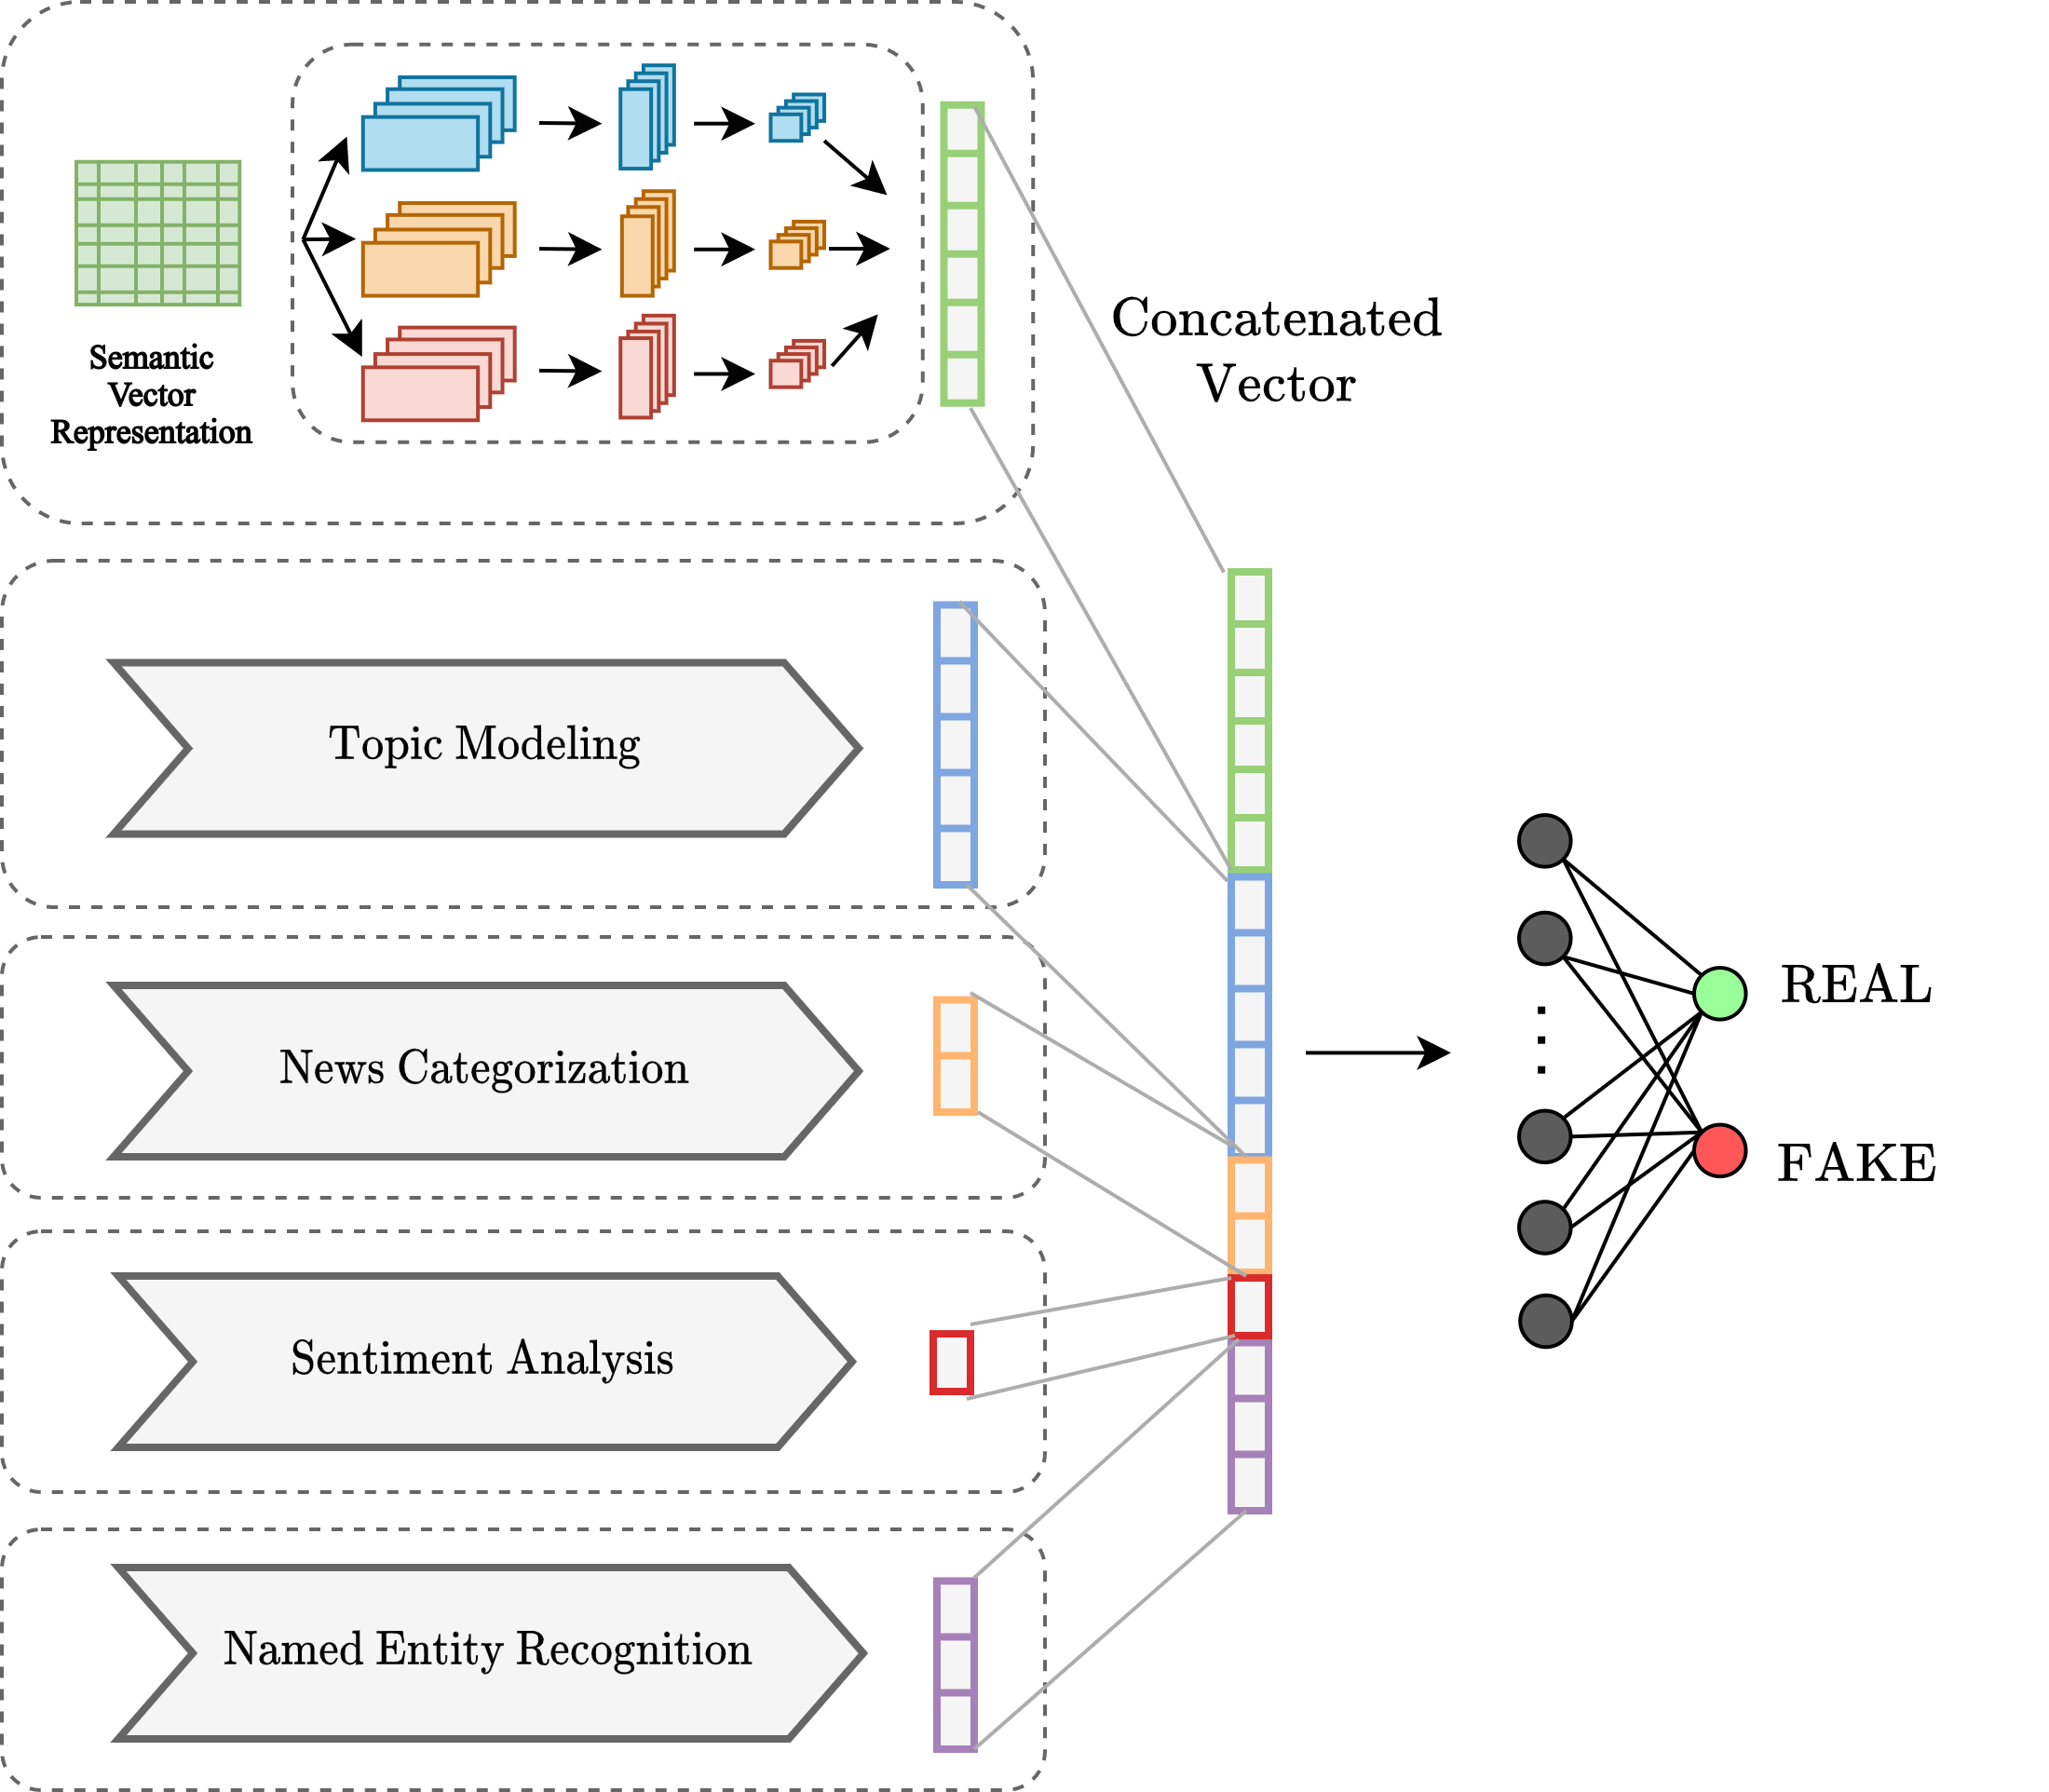
\includegraphics[width=0.75 \textwidth]{all_features}
	\centering
	\caption{شمای کلی مدل استفاده شده برای استفاده از تمام فراداده‌ها}
	\label{fig.all_features}
\end{figure}

\begin{figure}[h!]
	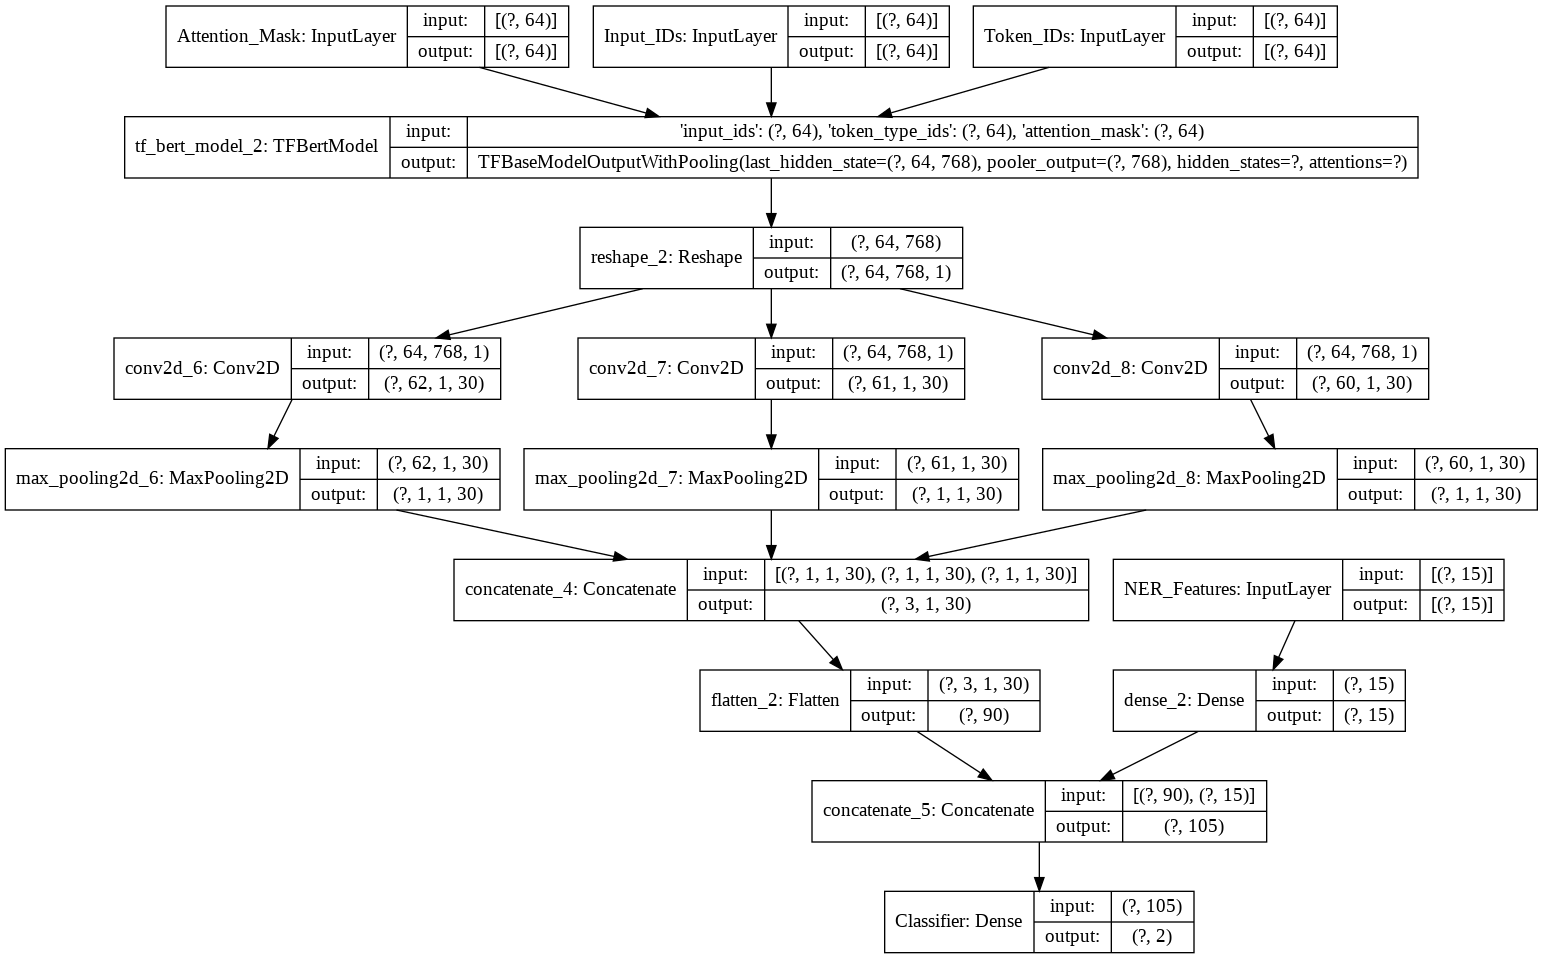
\includegraphics[width=1 \textwidth]{model_cnn_ner}
	\centering
	\caption{معماری مدل پیچشی با استفاده از فراداده موجودیت‌های نامدار}
	\label{fig.cnn_ner}
\end{figure}

جدول \ref{table.results_meta} نتایج حاصل از استفاده از هریک از فراداده‌های ذکرشده در کنار بازنمایی متنی  در دو شبکه پیچشی و پیشرو را نمایش می‌دهد. برای مقایسه راحت‌تر، نتایج حاصل از تشخیص اخبار بدون فراداده که در فصل قبل گزارش شده بود در این جدول تکرار شده‌است.
براساس جدول \ref{table.results_meta}، با استفاده از پردازش‌های متنی توانستیم دقت تشخیص اخبار جعلی را بهبود دهیم. همانطور که انتظار داشتیم دسته‌بند پیچشی توانست عملکرد بهتری را نسبت به مدل شبکه عصبی پرسپترون پیشرو داشته باشد. با توجه به نتایج، ازشمندترین فراداده که توانست دقت تشخیص مدل ما را بیشتر بهبود دهد، موضوع هر خبر (دسته‌بندی) بود که باعث افزایش \%$1.2$ معیار اف و \%$1.6$ دقت دسته‌بند پیچشی شد. این نتیجه دور از انتظار هم نبود چراکه موضوع هر خبر تاثیر بسیار زیادی در تشخیص اخبار جعلی دارد. همانطور که پیش از این هم اشاره شده، عمده اخبار جعلی در حوزه‌های سیاسی و اجتماعی منتشر می‌شوند. همچنین فراداده‌های مربوط به احساس‌ خبر، بردار موجودیت‌های نام‌د‌ار و موضوع (تخصیص نهان دیریکله) توانستند به طور مجزا دقت نهایی مدل را \%$0.5$، \%$1.35$ و \%$0.3$ افزایش دهند. در نهایت با استفاده از تمامی فراداده‌های استخراج شده از اخبار که با پیوستن به یکدیگر یک بردار ۷۳ بعدی را تشکیل دادند، مدل‌ پارس‌برت-پیچشی ارائه شده را ارزیابی کردیم که باعث افزایش ۲ درصدی معیار اف و دقت شد.

\begin{table}[h!]
	\caption{نتایج تشخیص اخبار جعلی فارسی با استفاده از بازنمایی پارس‌برت و دسته‌بندهای مختلف}
	\label{table.results_meta}
	\begin{center}
		\begin{tabular}{|c|c|c|c|c|c|c|}
			\hline
			بازنمائی & دسته‌بند & فراداده & فراخوانی & صحت & معیار اف & دقت \\
			\hline
			\hline
			\multirow{11}{*}{پارس‌برت} & \multirow{5}{*}{پیچشی}
			& - & $89.13$ & $93.71$ & $91.36$ & $91.64$ \\
			\cline{3-7}
			&  & موجودیت‌های نامدار & $91.16$& $94.28$ & $92.69$ & $92.99$ \\
		\cline{3-7}
			&  & احساس‌ خبر & $91.52$ & $92.57$ & $92.04$ & $92.45$ \\
			\cline{3-7}
			 &  & موضوع  (دسته‌بندی) & $96.87$ & $88.57$ & $92.53$ & $93.26$ \\
			\cline{3-7}
		 &  & موضوع  (تخصیص نهان دیریکله) & $91.42$ & $91.42$  & $91.42$  & $91.91$  \\
			\cline{3-7}
			&  & تمام ویژگی‌ها & $93.64$ & $92.57$ & $93.10$ & $93.53$ \\
			\cline{2-7}
			& \multirow{5}{*}{پرسپترون}
			& - & $92.44$ & $90.85$ & $91.64$ & $92.18$ \\
			\cline{3-7}
			&  &موجودیت‌های نامدار & $93.16$ & $85.71$ & $89.28$ & $90.29$ \\
			\cline{3-7}
			&  &احساس‌ خبر & $83.90$ & $98.28$ & $90.52 $ & $90.29$ \\
			\cline{3-7}
		&  & موضوع  (دسته‌بندی) & $89.13$ & $93.71$ & $91.36$ & $91.64$ \\
			\cline{3-7}
			&  & موضوع  (تخصیص نهان دیریکله)  & $87.89 $ & $95.42$ & $91.50$ & $91.64$ \\
			\hline
		\end{tabular}
	\end{center}
\end{table}